\documentclass[../entwurf.tex]{subfiles}

\begin{document}

\section{ViewModel}
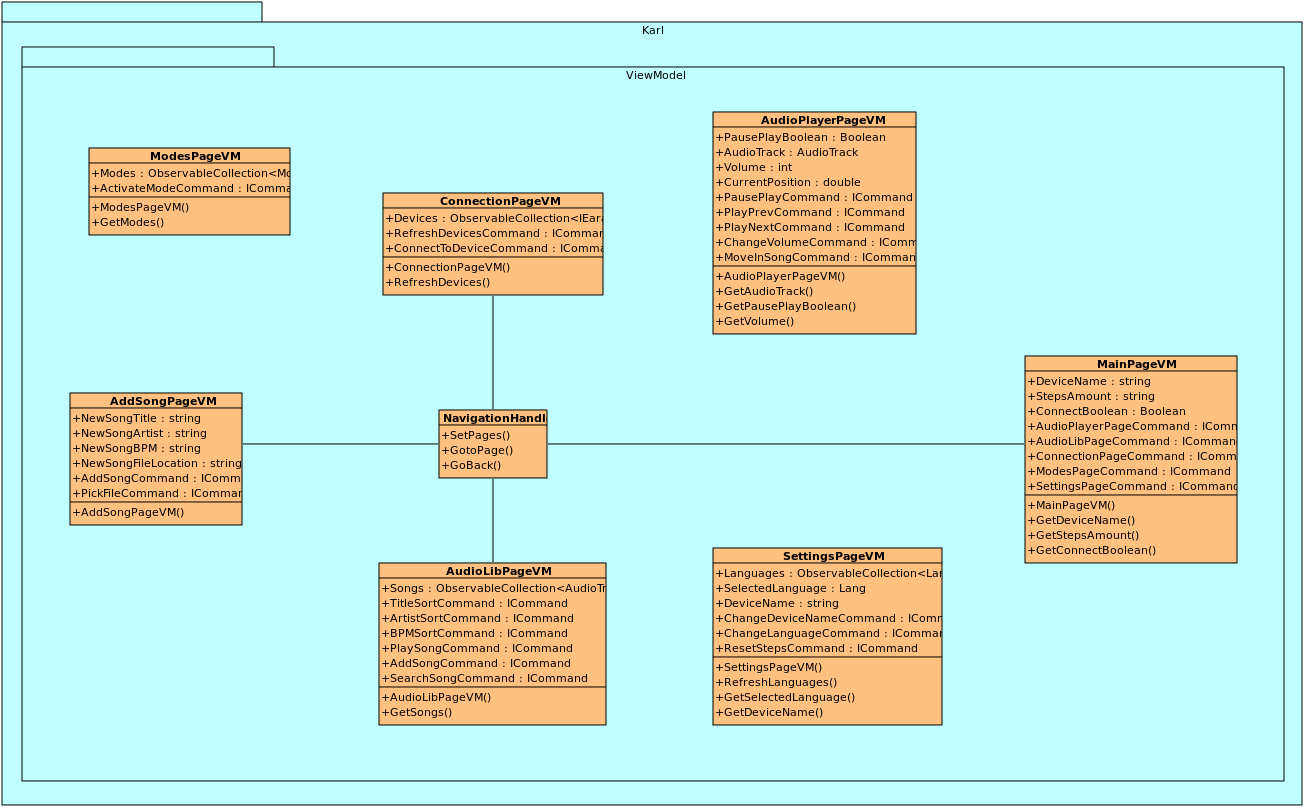
\includegraphics[scale=0.44,angle=90,origin=c]{../graphics/uml_diagramme/ViewModelDiagram.png}
\subsection{AddSongPageVM}
\begin{minipage}{0.45\textwidth}
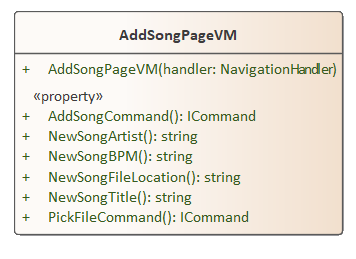
\includegraphics[scale=0.75]{../graphics/vm_klassen/AddSongPageVM.png}
\end{minipage}
\begin{minipage}{0.55\textwidth}
Diese Klasse enthält die UI-Logik der \code{AddSongPage}. Sie stellt dieser öffentliche Eigenschaften und Commands zur Verfügung, welche dort an Steuerelemente gebunden sind, um als Bindeglied zwischen der \code{AddSongPage} und dem Model zu dienen.
\end{minipage}
\paragraph{Attribute \& Properties}
\begin{itemize}
	\i{public string NewSongTitle} Hier wird der vom Nutzer eingegebene Titel eines Songs, der neu hinzugefügt werden soll, gespeichert.
	\i{public string NewSongArtist} Hier wird der vom Nutzer eingegebene Künstlername eines Songs, der neu hinzugefügt werden soll, gespeichert.
	\i{public string NewSongBPM} Hier wird der vom Nutzer eingegebene BPM-Wert eines Songs, der neu hinzugefügt werden soll, gespeichert.
	\i{public string NewSongFileLocation} Hier wird der vom Nutzer spezifizierte Pfad eines Songs, der neu hinzugefügt werden soll, gespeichert.
	\i{public ICommand\footnote{Stammt aus System.Windows.Input} AddSongCommand} Dieser Command fügt über private Methoden einen neuen Song zum Model hinzu, wobei \code{NewSongTitle}, \code{NewSongArtist}, \code{NewSongBPM} und \code{NewSongFileLocation} als Parameter dienen. \glsnote{ro}
	\i{public ICommand PickFileCommand} Dieser Command erlaubt es über private Methoden, dem Nutzer die Datei eines Songs aus dem Dateiensystem des Smartphones auszuwählen. \glsnote{ro}
\end{itemize}
\paragraph{Methoden}
\begin{itemize}
	\i{public AddSongPageVM(NavigationHandler handler)} Der Konstruktor der Klasse initialisiert die Commands.
\end{itemize}
\subsection{AudioLibPageVM}
\begin{minipage}{0.5\textwidth}
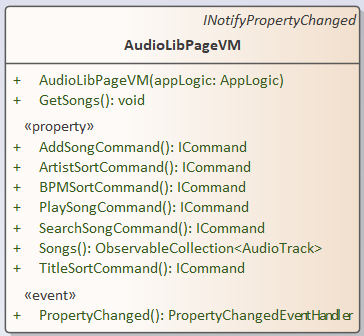
\includegraphics[scale=0.75]{../graphics/vm_klassen/AudioLibPageVM.png}
\end{minipage}
\begin{minipage}{0.5\textwidth}
Diese Klasse enthält die UI-Logik der \code{AudioLibPage}. Sie stellt dieser öffentliche Eigenschaften und Commands zur Verfügung, welche dort an Steuerelemente gebunden sind, um als Bindeglied zwischen der \code{AudioLibPage} und dem Model zu dienen.
\end{minipage}
\paragraph{Attribute \& Properties}
\begin{itemize}
	\i{public ObservableCollection<AudioTrack> Songs} Hier werden die Songs gespeichert, die in der View angezeigt werden sollen.
	\i{public ICommand TitleSortCommand} Dieser Command sortiert \code{Songs} alphabetisch nach Titel über private Methoden. \glsnote{ro}
	\i{public ICommand ArtistSortCommand} Dieser Command sortiert \code{Songs} alphabetisch nach Künstler über private Methoden. \glsnote{ro}
	\i{public ICommand BPMSortCommand} Dieser Command sortiert \code{Songs} aufsteigend nach BPM-Wert über private Methoden. \glsnote{ro}
	\i{public ICommand PlaySongCommand} Dieser Command spielt den in der View ausgewählten Song über private Methoden ab. \glsnote{ro}
	\i{public ICommand AddSongCommand} Dieser Command ermöglicht über private Methoden dem Nutzer, einen neuen Song zum Model hinzuzufügen. \glsnote{ro}
	\i{public ICommand SearchSongCommand} Dieser Command sucht im Model nach einem Song, dessen Titel, Künstler oder BPM-Wert mit dem in der View eingegeben Text in Teilen übereinstimmt. \glsnote{ro}
\end{itemize}
\paragraph{Methoden}
\begin{itemize}
	\i{public AudioLibPageVM(NavigationHandler handler)} Der Konstruktor der Klasse initialisiert die Commands.
	\i{public void GetSongs()} Diese Methode ruft die Songs ab, die im Model gespeichert sind und weist sie der Property \code{Songs} zu.
\end{itemize}
\subsection{AudioPlayerPageVM}
\begin{minipage}{0.5\textwidth}
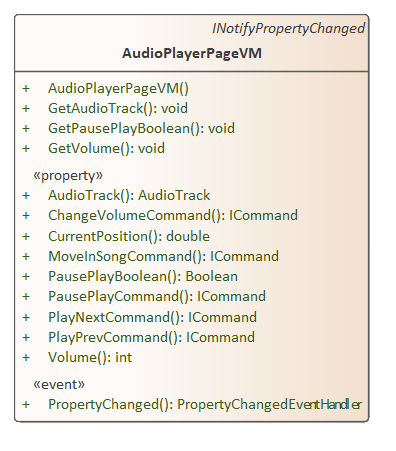
\includegraphics[scale=0.75]{../graphics/vm_klassen/AudioPlayerPageVM.png}
\end{minipage}
\begin{minipage}{0.5\textwidth}
Diese Klasse enthält die UI-Logik der \code{AudioPlayerPage}. Sie stellt dieser öffentliche Eigenschaften und Commands zur Verfügung, welche dort an Steuerelemente gebunden sind, um als Bindeglied zwischen der \code{AudioPlayerPage} und dem Model zu dienen.
\end{minipage}
\paragraph{Attribute \& Properties}
\begin{itemize}
	\i{public Boolean PausePlayBoolean} Dieser Boolean gibt an, ob der AudioPlayer im Model momentan aktiv oder pausiert ist.
	\i{public AudioTrack AudioTrack} Hier wird der momentan im Model geladene Song gespeichert.
	\i{public int Volume} Hier wird der Wert der Lautstärke gespeichert.
	\i{public double CurrentPosition} Hier wird die aktuelle Position im momentan aktiven Song gespeichert.
	\i{public Image Icon} Je nachdem ob der AudioPlayer aktiv oder pausiert ist, ist hier ein bestimmtes Bild gespeichert.
	\i{public ICommand PausePlayCommand} Dieser Command pausiert/spielt den momentan im Model geladenen Song über private Methoden. \glsnote{ro}
	\i{public ICommand PlayPrevCommand} Dieser Command spielt über private Methoden den Song ab, der sich im AudioPlayer des Models oben auf dem Stack befindet. \glsnote{ro}
	\i{public ICommand PlayNextCommand} Dieser Command spielt über private Methoden den Song ab, der sich im AudioPlayer des Models am Anfang der Queue befindet. \glsnote{ro}
	\i{public ICommand ChangeVolumeCommand} Dieser Command ändert die Laustärke im Model über private Methoden mit der in der View ausgewählten Lautstärke als Parameter.
	\i{public ICommand MoveInSongCommand} Dieser Command bewegt den Abspielzeitpunkt des momentan im Model geladenen Songs über private Methoden mit der in der View ausgewählten Position als Parameter.
\end{itemize}
\paragraph{Methoden}
\begin{itemize}
	\i{public AudioPlayerPageVM()} Der Konstruktor der Klasse initialisiert die Icons und die Commands.
	\i{public void GetAudioTrack()} Diese Methode ruft den im Model momentan geladenen Song ab und weist sie der Property \code{Songs} zu.
	\i{public void GetPausePlayBoolean()} Diese Methode ruft im Model ab, ob der Audioplayer aktiv oder pausiert werden soll und weist den Boolean der Property \code{PausePlayBoolean} zu.
	\i{public void GetVolume()} Diese Methode ruft im Model ab, ob der Audioplayer aktiv oder pausiert werden soll und weist den Boolean der Property \code{PausePlayBoolean} zu.
	\i{public event PropertyChangedEventHandler PropertyChanged} Dieser Eventhandler ermöglicht Kommunikation mit der View.
\end{itemize}
\subsection{ConnectionPageVM}
\begin{minipage}{0.5\textwidth}
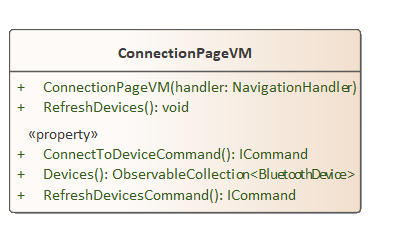
\includegraphics[scale=0.75]{../graphics/vm_klassen/ConnectionPageVM.png}
\end{minipage}
\begin{minipage}{0.5\textwidth}
Diese Klasse enthält die UI-Logik der \code{ConnectionPage}. Sie stellt dieser öffentliche Eigenschaften und Commands zur Verfügung, welche dort an Steuerelemente gebunden sind, um als Bindeglied zwischen der \code{ConnectionPage} und dem Model zu dienen.
\end{minipage}
\paragraph{Attribute \& Properties}
\begin{itemize}
	\i{public ObservableCollection<BluetoothDevice> Devices} Hier werden die Geräte gepeichert die in der View angezeigt werden sollen. \glsnote{ro}
	\i{public ICommand RefreshDevicesCommand} Dieser Command aktualisiert über private Methoden \code{Devices} mit den Geräten die im Model gefunden werden. \glsnote{ro}
	\i{public ICommand ConnectToDeviceCommand} Dieser Command versucht über private Methoden eine Verbindung mit dem in der View ausgewähltem Gerät aufzubauen. \glsnote{ro}
\end{itemize}
\paragraph{Methoden}
\begin{itemize}
	\i{public ConnectionPageVM(NavigationHandler handler)} Der Konstruktor der Klasse initialisiert die Commands.
	\i{public void RefreshDevices()} Diese Methode ruft die im Model momentan erkannten Geräte ab und fügt sie der Property \code{Devices} hinzu.
\end{itemize}
\subsection{MainPageVM}
\begin{minipage}{0.5\textwidth}
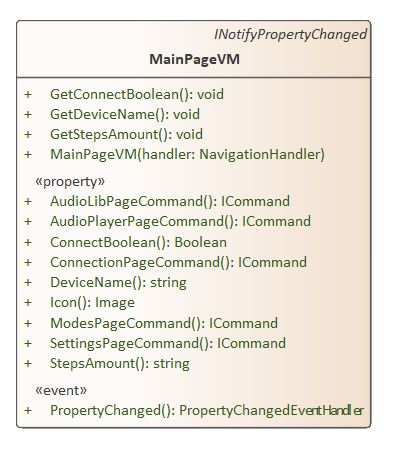
\includegraphics[scale=0.75]{../graphics/vm_klassen/MainPageVM.png}
\end{minipage}
\begin{minipage}{0.5\textwidth}
Diese Klasse enthält die UI-Logik der \code{MainPage}. Sie stellt dieser öffentliche Eigenschaften und Commands zur Verfügung, welche dort an Steuerelemente gebunden sind, um als Bindeglied zwischen der \code{MainPage} und dem Model zu dienen.
\end{minipage}
\paragraph{Attribute \& Properties}
\begin{itemize}
	\i{public string DeviceName} Hier wird der Name des momentan verbundenen Geräts gespeichert, falls keine Verbindung besteht, hat der String den wert null.
	\i{public string StepsAmount} Hier wird die Anzahl der Schritte seit dem letzten Reset gespeichert, falls keine Verbindung zu einem Gerät besteht, hat der String den wert null.
	\i{public Boolean ConnectBoolean} Dieser Boolean gibt an, ob eine Verbindung zu einem Gerät besteht.
	\i{public Image Icon} Je nachdem ob eine Verbindung zu einem Gerät besteht oder nicht, ist hier ein bestimmtes Bild gespeichert.
	\i{public ICommand AudioPlayerPageCommand} Dieser Command ändert die Ansicht der App über private Methoden zur AudioPlayerPage. \glsnote{ro}
	\i{public ICommand AudioLibPageCommand} Dieser Command ändert die Ansicht der App über private Methoden zur AudioLibPage. \glsnote{ro}
	\i{public ICommand ConnectionPageCommand} Dieser Command ändert die Ansicht der App über private Methoden zur ConnectionPage. \glsnote{ro}
	\i{public ICommand ModesPageCommand} Dieser Command ändert die Ansicht der App über private Methoden zur ModesPage. \glsnote{ro}
	\i{public ICommand SettingsPageCommand} Dieser Command ändert die Ansicht der App über private Methoden zur SettingsPage. \glsnote{ro}
\end{itemize}
\paragraph{Methoden}
\begin{itemize}
	\i{public MainPageVM(AppLogic appLogic)} Der Konstruktor der Klasse initialisiert die Icons und die Commands.
	\i{public void GetDeviceName()} Diese Methode ruft den Namen des momentan verbundenen Gerätes im Model ab und weist sie der Property \code{DeviceName} zu.
	\i{public void GetStepsAmount()} Diese Methode ruft im Model ab, wie viele Schritte seit dem letztem Reset gemacht wurden und weist den Wert der Property \code{StepsAmount} zu.
	\i{public void GetConnectBoolean()} Diese Methode ruft im Model ab, ob momentan eine Verbindung zu einem Gerät besteht und weist den Boolean der Property \code{ConnectBoolean} zu.
	\i{public event PropertyChangedEventHandler PropertyChanged} Dieser Eventhandler ermöglicht Kommunikation mit der View.
\end{itemize}
\subsection{ModesPageVM}
\begin{minipage}{0.5\textwidth}
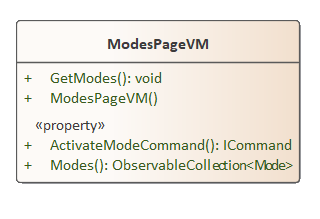
\includegraphics[scale=0.75]{../graphics/vm_klassen/ModesPageVM.png}
\end{minipage}
\begin{minipage}{0.5\textwidth}
Diese Klasse enthält die UI-Logik der \code{ModesPage}. Sie stellt dieser öffentliche Eigenschaften und Commands zur Verfügung, welche dort an Steuerelemente gebunden sind, um als Bindeglied zwischen der \code{ModesPage} und dem Model zu dienen.
\end{minipage}
\paragraph{Attribute \& Properties}
\begin{itemize}
	\i{public ObservableCollection<Mode> Modes} Hier werden die Modi gespeichert, die in der View angezeigt werden sollen.
	\i{public ICommand ActivateModeCommand} Dieser Command aktiviert über private Methoden im Model den in der View ausgewählten Modus. \glsnote{ro}
\end{itemize}
\paragraph{Methoden}
\begin{itemize}
	\i{public ModesPageVM()} Der Konstruktor der Klasse initialisiert die Commands.
	\i{public void GetModes()} Diese Methode ruft die im Model vorhandenen Modi ab und weist sie der Property \code{Modes} zu.
\end{itemize}
\subsection{SettingsPageVM}
\begin{minipage}{0.5\textwidth}
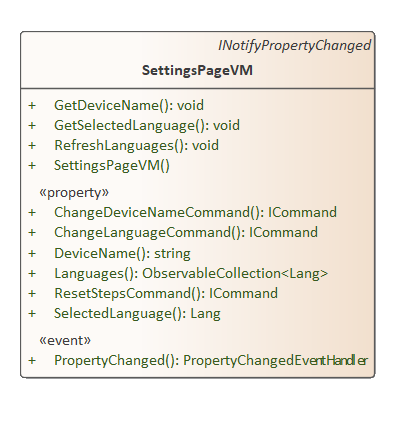
\includegraphics[scale=0.75]{../graphics/vm_klassen/SettingsPageVM.png}
\end{minipage}
\begin{minipage}{0.5\textwidth}
Diese Klasse enthält die UI-Logik der \code{SettingsPage}. Sie stellt dieser öffentliche Eigenschaften und Commands zur Verfügung, welche dort an Steuerelemente gebunden sind, um als Bindeglied zwischen der \code{SettingsPage} und dem Model zu dienen.
\end{minipage}
\paragraph{Attribute \& Properties}
\begin{itemize} 
	\i{public ObservableCollection<Lang> Languages} Hier werden die Sprachen gespeichert, die in der View angezeigt werden sollen.
	\i{public Lang SelectedLanguage} Hier wird die Sprache gespeichert, die in der View als ausgewählt angezeigt wird.
	\i{public string DeviceName} Hier wird der Name des momentan verbundenen Geräts gepeichert der in der View angezeigt wird.
	\i{public ICommand ChangeDeviceNameCommand} Dieser Command setzt über private Methoden im Model den Namen des Geräts auf den in der View eingegebenen Text. \glsnote{ro}
	\i{public ICommand ChangeLanguageCommand} Dieser Command ändert über private Methoden im Model die Sprache auf die in der View ausgewählten Sprache. \glsnote{ro}
	\i{public ICommand ResetStepsCommand} Dieser Command setzt über private Methoden die Schrittanzahl im Model zurück. \glsnote{ro}
\end{itemize}
\paragraph{Methoden}
\begin{itemize}
	\i{public SettingsPageVM()} Der Konstruktor der Klasse initialisiert die Commands.
	\i{public void RefreshLanguages()} Diese Methode ruft die im Model vorhandenen Sprachen ab und weist sie der Property \code{Languages} zu.
	\i{public void GetSelectedLanguage()} Diese Methode ruft die im Model ausgewählte Sprache ab und weist sie der Property \code{SelectedLanguage} zu.
	\i{public void GetDeviceName()} Diese Methode ruft den Namen des momentan verbundenen Gerätes im Model ab und weist ihn der Property \code{DeviceName} zu.
	\i{public event PropertyChangedEventHandler PropertyChanged} Dieser Eventhandler ermöglicht Kommunikation mit der View.
\end{itemize}
\subsection{NavigationHandler}
\begin{minipage}{0.45\textwidth}
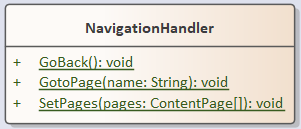
\includegraphics[scale=0.75]{../graphics/vm_klassen/NavigationHandler.png}
\end{minipage}
\begin{minipage}{0.55\textwidth}
Diese Klasse ermöglicht den verschiedenen Klassen der ViewModels die Ansicht der App auf andere ContentPages der View zu ändern.
\end{minipage}
\paragraph{Attribute \& Properties}
\paragraph{Methoden}
\begin{itemize}
	\i{public void SetPages(ContentPage[] pages)} Diese Methode speichert das übergebene Array in der Klasse ab.
	\i{public async void GotoPage(String name)} Diese Methode ändert die Ansicht der App auf die ContentPage deren Namen dem übergebenen String entspricht.
	\i{public async void GoBack()} Diese Methode ändert die Ansicht der App auf die ContentPage die zuvor angezeigt wurde.
\end{itemize}

\end{document}
